\documentclass[aspectratio=169,10pt]{beamer}

\usepackage[T1]{fontenc}
\usepackage[utf8]{inputenc}
\usepackage{lmodern}
\usepackage{amsmath,amssymb}
\usepackage{graphicx}
\usepackage{booktabs}
\usepackage{array}
\usepackage{ragged2e}
\usepackage{xcolor}
\usepackage{microtype}
\usepackage{tikz}
\usepackage{listings}
\usetikzlibrary{positioning,arrows.meta,calc,shapes.geometric,shadows.blur}

% ---------- Unified palette ----------
\definecolor{IQMnavy}{HTML}{102033}
\definecolor{IQMblue}{HTML}{2A6F97}
\definecolor{IQMblueDark}{HTML}{245C7F}
\definecolor{IQMlight}{HTML}{F4F7FA}
\definecolor{IQMmuted}{HTML}{667085}
\definecolor{IQMline}{HTML}{D0D5DD}
\definecolor{IQMaccent}{HTML}{E9F4FB}
\definecolor{IQMgreen}{HTML}{2E7D60}
\definecolor{IQMamber}{HTML}{B7791F}
\definecolor{IQMred}{HTML}{A64B4B}
\definecolor{IQMcode}{HTML}{EEF4FF}
\definecolor{IQMpaper}{HTML}{FBFCFE}

\setbeamercolor{background canvas}{bg=white}
\setbeamertemplate{navigation symbols}{}
\setbeamertemplate{headline}{}
\setbeamertemplate{frametitle}{%
  \vspace{0.22cm}\insertframetitle\par\vspace{0.06cm}%
  {\color{IQMblue}\rule{0.78cm}{1.5pt}}\vspace{0.10cm}}
\setbeamertemplate{footline}{%
  \leavevmode%
  \hbox{%
  \begin{beamercolorbox}[wd=.78\paperwidth,ht=2.4ex,dp=1.1ex,leftskip=1.2em]{footline}%
    \tiny\textcolor{IQMmuted}{Compression pipeline | fixed target sizes | no-reference IQMs}%
  \end{beamercolorbox}%
  \begin{beamercolorbox}[wd=.22\paperwidth,ht=2.4ex,dp=1.1ex,rightskip=1.2em plus1fil]{footline}%
    \tiny\hfill\textcolor{IQMmuted}{\insertframenumber/\inserttotalframenumber}%
  \end{beamercolorbox}}%
}

\setbeamercolor{frametitle}{fg=IQMnavy,bg=white}
\setbeamerfont{frametitle}{series=\bfseries,size=\large}
\setbeamercolor{title}{fg=IQMnavy}
\setbeamerfont{title}{series=\bfseries,size=\LARGE}
\setbeamercolor{subtitle}{fg=IQMmuted}
\setbeamerfont{subtitle}{size=\large}
\setbeamercolor{normal text}{fg=IQMnavy,bg=white}
\setbeamercolor{item}{fg=IQMblue}
\setbeamerfont{itemize/enumerate body}{size=\footnotesize}
\setbeamerfont{itemize/enumerate subbody}{size=\scriptsize}
\setlength{\parskip}{0.18em}
\setlength{\fboxsep}{0pt}
\setlength{\parindent}{0pt}

% ---------- Listings ----------
\lstdefinestyle{py}{
  language=Python,
  basicstyle=\ttfamily\scriptsize,
  keywordstyle=\bfseries\color{IQMblueDark},
  commentstyle=\color{IQMmuted},
  stringstyle=\color{IQMgreen},
  showstringspaces=false,
  columns=fullflexible,
  keepspaces=true,
  breaklines=true,
  breakatwhitespace=true,
  backgroundcolor=\color{IQMcode},
  frame=single,
  rulecolor=\color{IQMline},
  framerule=0.5pt,
  xleftmargin=4pt,
  xrightmargin=4pt,
  aboveskip=4pt,
  belowskip=2pt
}

% ---------- Helpers ----------
\newcommand{\slidetag}[1]{\vspace{0.05em}{\scriptsize\textcolor{IQMblue}{\textbf{#1}}}\vspace{0.16em}}
\newcommand{\source}[1]{\vspace{0.08em}{\tiny\textcolor{IQMmuted}{Source: #1}}}
\newcommand{\paperfig}[3]{%
  \begin{center}
    \fcolorbox{IQMline}{white}{\includegraphics[width=#2,height=#3,keepaspectratio]{#1}}
  \end{center}
}
\newcommand{\legenditem}[2]{\textcolor{IQMblue}{\textbf{#1}}\, #2}
\newcommand{\smallmuted}[1]{{\color{IQMmuted}\footnotesize #1}}

\tikzset{
  flowbox/.style={rounded corners=2.6pt, draw=IQMblue!60, fill=IQMaccent, thick, align=center, minimum height=0.52cm, font=\scriptsize\bfseries, text=IQMnavy, inner xsep=5pt},
  flowarr/.style={-{Latex[length=2.2mm]}, thick, draw=IQMblueDark},
  metricbox/.style={rounded corners=3pt, draw=IQMline, fill=IQMlight, align=left, inner sep=6pt},
  callout/.style={rounded corners=3pt, draw=IQMblue!55, fill=IQMaccent, align=center, inner sep=6pt},
  card/.style={rounded corners=5pt, draw=IQMline, fill=white, align=left, inner sep=7pt, text=IQMnavy},
  softcard/.style={rounded corners=5pt, draw=IQMblue!35, fill=IQMaccent, align=center, inner sep=6pt, text=IQMnavy},
  ambercard/.style={rounded corners=5pt, draw=IQMamber!45, fill=IQMamber!8, align=center, inner sep=6pt, text=IQMnavy},
  greencard/.style={rounded corners=5pt, draw=IQMgreen!45, fill=IQMgreen!8, align=center, inner sep=6pt, text=IQMnavy}
}

\newcommand{\flowthree}[3]{%
\vspace{0.05em}\begin{center}\resizebox{0.96\linewidth}{!}{%
\begin{tikzpicture}[node distance=0.9cm]
\node[flowbox, minimum width=3.1cm] (a) {#1};
\node[flowbox, minimum width=3.1cm, right=of a] (b) {#2};
\node[flowbox, minimum width=3.1cm, right=of b] (c) {#3};
\draw[flowarr] (a) -- (b); \draw[flowarr] (b) -- (c);
\end{tikzpicture}}\end{center}}
\newcommand{\flowfour}[4]{%
\vspace{0.05em}\begin{center}\resizebox{0.96\linewidth}{!}{%
\begin{tikzpicture}[node distance=0.75cm]
\node[flowbox, minimum width=2.55cm] (a) {#1};
\node[flowbox, minimum width=2.55cm, right=of a] (b) {#2};
\node[flowbox, minimum width=2.55cm, right=of b] (c) {#3};
\node[flowbox, minimum width=2.55cm, right=of c] (d) {#4};
\draw[flowarr] (a) -- (b); \draw[flowarr] (b) -- (c); \draw[flowarr] (c) -- (d);
\end{tikzpicture}}\end{center}}
\newcommand{\flowfive}[5]{%
\vspace{0.05em}\begin{center}\resizebox{0.96\linewidth}{!}{%
\begin{tikzpicture}[node distance=0.55cm]
\node[flowbox, minimum width=2.35cm] (a) {#1};
\node[flowbox, minimum width=2.35cm, right=of a] (b) {#2};
\node[flowbox, minimum width=2.35cm, right=of b] (c) {#3};
\node[flowbox, minimum width=2.35cm, right=of c] (d) {#4};
\node[flowbox, minimum width=2.35cm, right=of d] (e) {#5};
\draw[flowarr] (a) -- (b); \draw[flowarr] (b) -- (c); \draw[flowarr] (c) -- (d); \draw[flowarr] (d) -- (e);
\end{tikzpicture}}\end{center}}

\title{Compression Pipeline \& No-Reference IQA}
\subtitle{Placeholder title page}
\author{PS Multimediale Datenformate SS2026}
\date{}

\begin{document}

% ---------- Slide 1: placeholder title ----------
\begin{frame}[plain]
  
\begin{tikzpicture}[remember picture,overlay]
    \fill[IQMpaper] (current page.south west) rectangle (current page.north east);
    \fill[IQMaccent] (current page.south west) rectangle ($(current page.south west)+(3.0,9)$);
    \fill[IQMblue!12] ($(current page.south east)+(-2.0,0)$) rectangle (current page.north east);
    \node[anchor=west, text=IQMnavy, font=\bfseries\fontsize{26}{31}\selectfont] at (-0.1,1.20) {Presentation title};
    \node[anchor=west, text=IQMmuted, font=\fontsize{15}{18}\selectfont] at (-0.1,0.55) {placeholder - final title page to be added later};
    \node[anchor=west, text=IQMblueDark, font=\small\bfseries] at (-0.1,-0.15) {Compression pipeline + no-reference IQMs};
    \node[anchor=west, text=IQMmuted, font=\scriptsize] at (-0.1,-3.05) {JPEG · JPEG2000 · JPEG XR · JPEG XL · JPEG AI  /  BRISQUE · NIQE · NIMA · CLIP-IQA};
  \end{tikzpicture}
\end{frame}

% ---------- Slide 2: compression experiment ----------
\begin{frame}{Compression experiment: workflow and objective}
\begin{columns}[T,onlytextwidth]
  \begin{column}{0.48\textwidth}
    \slidetag{Task performed}
    \begin{itemize}\setlength\itemsep{0.36em}
      \item Selected representative \textbf{600 $\times$ 600} test images.
      \item Compressed each image with \textbf{JPEG, JPEG2000, JPEG XR, JPEG XL, JPEG AI}.
      \item Used fixed target filesizes: \textbf{175, 150, 125, 100, 75, 50, 25 kB}.
      \item Assessed all outputs with \textbf{BRISQUE, NIQE, NIMA, CLIP-IQA}.
    \end{itemize}
  \end{column}
  \begin{column}{0.48\textwidth}
    \slidetag{Why this was done}
    \begin{itemize}\setlength\itemsep{0.36em}
      \item Identify suitable codecs for different byte budgets.
      \item Study quality changes under strong compression.
      \item Check whether no-reference IQMs capture compression artefacts.
      \item Support codec comparison without reference images.
    \end{itemize}
  \end{column}
\end{columns}
\vspace{0.24cm}
\begin{center}
\resizebox{0.96\linewidth}{!}{%

\begin{tikzpicture}[node distance=0.48cm]
  \node[flowbox, minimum width=2.25cm, minimum height=0.85cm, fill=IQMlight] (a) {test images\\[-0.1em]\scriptsize 600 $\times$ 600};
  \node[flowbox, minimum width=2.65cm, minimum height=0.85cm, right=of a] (b) {compress\\[-0.1em]\scriptsize 5 standards};
  \node[flowbox, minimum width=3.15cm, minimum height=0.85cm, right=of b, fill=IQMaccent] (c) {fixed target sizes\\[-0.1em]\scriptsize 175 to 25 kB};
  \node[flowbox, minimum width=2.85cm, minimum height=0.85cm, right=of c] (d) {assess\\[-0.1em]\scriptsize 4 IQMs};
  \node[flowbox, minimum width=2.75cm, minimum height=0.85cm, right=of d, fill=IQMgreen!10, draw=IQMgreen!45] (e) {analyse\\[-0.1em]\scriptsize suitability + artefacts};
  \draw[flowarr] (a) -- (b); \draw[flowarr] (b) -- (c); \draw[flowarr] (c) -- (d); \draw[flowarr] (d) -- (e);
\end{tikzpicture}}
\end{center}
\vfill
\begin{center}

\begin{tikzpicture}
  \node[card, text width=0.88\linewidth, align=center] {\footnotesize At small filesizes, visible compression artefacts are expected; the IQMs should reflect these degradations.};
\end{tikzpicture}
\end{center}
\end{frame}

% ---------- Slide 3: IQM divider ----------
\begin{frame}{No-reference image quality metrics}
  \begin{center}
    \vspace{0.50cm}
    {\usebeamerfont{title}\textcolor{IQMnavy}{BRISQUE, NIQE, NIMA, CLIP-IQA}}\\[0.5em]
    {\usebeamerfont{subtitle}\textcolor{IQMmuted}{Natural statistics, rating distributions and vision-language similarity}}\\[0.95cm]
    
\begin{tikzpicture}
      \node[flowbox, minimum width=3.25cm, minimum height=0.85cm] (a) {Natural scene\\statistics};
      \node[flowbox, minimum width=3.25cm, minimum height=0.85cm, right=0.9cm of a] (b) {Neural rating\\distributions};
      \node[flowbox, minimum width=3.25cm, minimum height=0.85cm, right=0.9cm of b] (c) {Vision-language\\similarity};
      \draw[flowarr] (a) -- (b); \draw[flowarr] (b) -- (c);
    \end{tikzpicture}
    \vfill
    {\tiny\textcolor{IQMmuted}{Primary sources: Mittal et al. 2012; Mittal et al. 2013; Talebi and Milanfar 2018; Wang et al. 2023}}
  \end{center}
\end{frame}

% ---------- Slide 4 ----------
\begin{frame}{Common framing: no-reference IQA}
\begin{columns}[T,onlytextwidth]
  \begin{column}{0.50\textwidth}
    \vspace{0.05cm}
    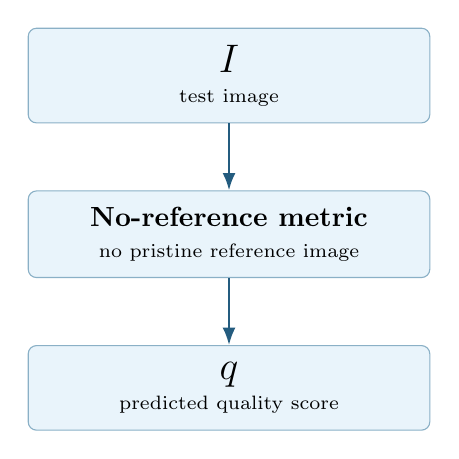
\begin{tikzpicture}[node distance=0.85cm]
      \node[callout, minimum width=5.1cm, minimum height=0.9cm] (i) {\Large\(I\)\\[-0.1em]\scriptsize test image};
      \node[callout, minimum width=5.1cm, minimum height=0.9cm, below=of i] (m) {\textbf{No-reference metric}\\[-0.1em]\scriptsize no pristine reference image};
      \node[callout, minimum width=5.1cm, minimum height=0.9cm, below=of m] (q) {\Large\(q\)\\[-0.1em]\scriptsize predicted quality score};
      \draw[flowarr] (i) -- (m); \draw[flowarr] (m) -- (q);
    \end{tikzpicture}
  \end{column}
  \begin{column}{0.46\textwidth}
    \slidetag{Scope}
    \begin{itemize}
      \item Image quality assessment predicts perceived image quality.
      \item No-reference IQA uses only the test image.
      \item BRISQUE and NIQE use natural scene statistics.
      \item NIMA uses human rating distributions.
      \item CLIP-IQA uses image-text similarity.
    \end{itemize}
  \end{column}
\end{columns}
\vfill
\flowthree{image}{metric}{quality score}
\end{frame}

% ---------- Slide 5 ----------
\begin{frame}{BRISQUE: core idea}
\begin{columns}[T,onlytextwidth]
  \begin{column}{0.54\textwidth}
    \paperfig{assets/brisque_fig4_hist.png}{\linewidth}{0.55\textheight}
    \source{Mittal, Moorthy, and Bovik (2012), Fig. 4.}
  \end{column}
  \begin{column}{0.42\textwidth}
    \slidetag{Method facts}
    \begin{itemize}
      \item Works directly in the spatial domain.
      \item Uses locally normalized luminance coefficients.
      \item Models MSCN coefficients with a GGD.
      \item Models neighboring MSCN products in four directions.
      \item Maps features to quality using SVR.
    \end{itemize}
  \end{column}
\end{columns}
\vfill
\flowfive{input image}{MSCN}{GGD/AGGD features}{SVR}{quality score}
\end{frame}

% ---------- Slide 6 ----------
\begin{frame}{BRISQUE: formula and pipeline}
\begin{columns}[T,onlytextwidth]
  \begin{column}{0.48\textwidth}
    \paperfig{assets/brisque_fig3_mscn.png}{\linewidth}{0.57\textheight}
    \source{Mittal, Moorthy, and Bovik (2012), Fig. 3.}
  \end{column}
  \begin{column}{0.48\textwidth}
    \slidetag{MSCN coefficient}
    \vspace{-0.3em}
    \begin{equation*}
      \hat{I}(i,j)=\frac{I(i,j)-\mu(i,j)}{\sigma(i,j)+C}
    \end{equation*}
    \vspace{-0.5em}
    {\scriptsize
    \begin{itemize}
      \item \legenditem{\(I(i,j)\):}{luminance value.}
      \item \legenditem{\(\mu(i,j)\):}{local mean.}
      \item \legenditem{\(\sigma(i,j)\):}{local contrast.}
      \item \legenditem{\(\hat{I}(i,j)\):}{MSCN coefficient.}
      \item \legenditem{\(C\):}{stabilizing constant.}
    \end{itemize}}
    \vspace{0.1em}
    \slidetag{Neighbor products}
    {\scriptsize\[
      H=\hat I(i,j)\hat I(i,j+1),\quad
      V=\hat I(i,j)\hat I(i+1,j)
    \]}
  \end{column}
\end{columns}
\vfill
\flowfour{image}{local normalization}{MSCN statistics}{feature vector}
\end{frame}

% ---------- Slide 7 ----------
\begin{frame}{NIQE: core idea}
\begin{columns}[T,onlytextwidth]
  \begin{column}{0.54\textwidth}
    \vspace{0.25cm}
    \paperfig{assets/niqe_patches.png}{0.86\linewidth}{0.40\textheight}
    \source{Mittal, Soundararajan, and Bovik (2013), Fig. 1.}
  \end{column}
  \begin{column}{0.42\textwidth}
    \slidetag{Method facts}
    \begin{itemize}
      \item NIQE is called ``completely blind.''
      \item It uses no human-rated distorted images.
      \item It uses no exposure to distorted images.
      \item It learns NSS features from natural images.
      \item Quality is distance to the natural MVG model.
    \end{itemize}
  \end{column}
\end{columns}
\vfill
\flowfour{natural image corpus}{patch features}{pristine MVG}{distance model}
\end{frame}

% ---------- Slide 8 ----------
\begin{frame}{NIQE: formula and pipeline}
\begin{columns}[T,onlytextwidth]
  \begin{column}{0.44\textwidth}
    \vspace{0.12cm}
    \begin{center}
    
\begin{tikzpicture}[node distance=0.78cm]
      \node[draw=IQMblue, fill=IQMaccent, very thick, ellipse,
            minimum width=2.25cm, minimum height=1.10cm] (P) {};
      \node[draw=IQMmuted, fill=IQMlight, very thick, ellipse,
            minimum width=2.25cm, minimum height=1.10cm,
            right=of P] (T) {};
      \node[circle, fill=IQMblue, inner sep=2.0pt] at (P.center) {};
      \node[circle, fill=IQMmuted, inner sep=2.0pt] at (T.center) {};
      \node[text=IQMblue, font=\scriptsize\bfseries] at ($(P.center)+(0,0.33)$) {\(\mu_p\)};
      \node[text=IQMmuted, font=\scriptsize\bfseries] at ($(T.center)+(0,0.33)$) {\(\mu_d\)};
      \node[text=IQMblue, font=\scriptsize\bfseries, align=center] at ($(P.south)+(0,-0.28)$) {Pristine MVG};
      \node[text=IQMmuted, font=\scriptsize\bfseries, align=center] at ($(T.south)+(0,-0.28)$) {Test-image MVG};
      \draw[flowarr] (P.center) -- node[above, font=\scriptsize, text=IQMnavy]{distance \(D\)} (T.center);
    \end{tikzpicture}
    \end{center}
    \vspace{0.35cm}
    \begin{center}
    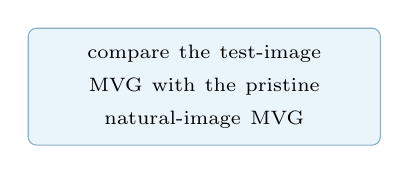
\begin{tikzpicture}
      \node[callout, text width=4.05cm, align=center]
      {\scriptsize compare the test-image MVG with the pristine natural-image MVG};
    \end{tikzpicture}
    \end{center}
  \end{column}
  \begin{column}{0.52\textwidth}
    \slidetag{NIQE distance}
    \begin{center}
    \resizebox{0.96\linewidth}{!}{$
    D=\sqrt{(\mu_p-\mu_d)^T
    \left(\frac{\Sigma_p+\Sigma_d}{2}\right)^{-1}
    (\mu_p-\mu_d)}
    $}
    \end{center}
    \vspace{-0.5em}
    {\scriptsize
    \begin{itemize}
      \item \legenditem{\(\mu_p,\Sigma_p\):}{pristine natural-image MVG.}
      \item \legenditem{\(\mu_d,\Sigma_d\):}{test-image MVG.}
      \item \legenditem{\(D\):}{NIQE distance score.}
      \item Lower distance means closer to pristine statistics.
    \end{itemize}}
  \end{column}
\end{columns}
\vfill
\flowfive{image}{MSCN patches}{NSS features}{test MVG}{distance \(D\)}
\end{frame}

% ---------- Slide 9 ----------
\begin{frame}{NIMA: core idea}
\begin{columns}[T,onlytextwidth]
  \begin{column}{0.54\textwidth}
    \paperfig{assets/nima_fig1_ratings.png}{\linewidth}{0.30\textheight}
    \vspace{0.10cm}
    \paperfig{assets/nima_fig2_examples.png}{\linewidth}{0.21\textheight}
    \source{Talebi and Milanfar (2018), Figs. 1--2.}
  \end{column}
  \begin{column}{0.42\textwidth}
    \slidetag{Method facts}
    \begin{itemize}
      \item NIMA uses a convolutional neural network.
      \item It predicts a distribution of human scores.
      \item It does not predict only the mean score.
      \item It uses no golden reference image.
      \item It supports no-reference perceptual assessment.
    \end{itemize}
  \end{column}
\end{columns}
\vfill
\flowfour{image}{CNN}{rating distribution}{mean + variance}
\end{frame}

% ---------- Slide 10 ----------
\begin{frame}{NIMA: formula and pipeline}
\begin{columns}[T,onlytextwidth]
  \begin{column}{0.48\textwidth}
    \vspace{0.15cm}
    \paperfig{assets/nima_fig8_architecture.png}{\linewidth}{0.22\textheight}
    \vspace{0.2cm}
    \paperfig{assets/nima_fig9_pred_gt.png}{0.82\linewidth}{0.20\textheight}
    \source{Talebi and Milanfar (2018), Figs. 8--9.}
  \end{column}
  \begin{column}{0.48\textwidth}
    \slidetag{Distribution output}
    {\scriptsize
    \begin{equation*}
      \hat{p}_i=\frac{e^{z_i}}{\sum_{j=1}^{N}e^{z_j}},\qquad
      \hat{\mu}=\sum_{i=1}^{N}s_i\hat{p}_i
    \end{equation*}
    \begin{equation*}
      \hat{\sigma}^{2}=\sum_{i=1}^{N}(s_i-\hat{\mu})^2\hat{p}_i
    \end{equation*}}
    \vspace{-0.45em}
    {\scriptsize
    \begin{itemize}
      \item \legenditem{\(z_i\):}{network logit.}
      \item \legenditem{\(\hat{p}_i\):}{predicted score probability.}
      \item \legenditem{\(s_i\):}{rating value.}
      \item \legenditem{\(\hat{\mu}\):}{predicted mean score.}
      \item \legenditem{\(\hat{\sigma}^{2}\):}{predicted score variance.}
    \end{itemize}}
  \end{column}
\end{columns}
\vfill
\flowfive{image}{CNN logits}{softmax}{rating distribution}{mean/variance}
\end{frame}

% ---------- Slide 11 ----------
\begin{frame}{NIMA: training loss}
\begin{columns}[T,onlytextwidth]
  \begin{column}{0.48\textwidth}
    \vspace{0.08cm}
    \paperfig{assets/nima_fig14_enhancement.png}{0.70\linewidth}{0.49\textheight}
    \source{Talebi and Milanfar (2018), Fig. 14.}
  \end{column}
  \begin{column}{0.48\textwidth}
    \slidetag{EMD facts}
    \begin{itemize}
      \item Ratings are ordered classes.
      \item The model predicts score probabilities.
      \item Training compares predicted and true distributions.
      \item NIMA uses Earth Mover's Distance.
      \item EMD measures distribution closeness.
    \end{itemize}
    \vspace{0.05em}
    {\scriptsize
    \[
    EMD(p,\hat p)=\left(\frac{1}{N}\sum_{k=1}^{N}|CDF_p(k)-CDF_{\hat p}(k)|^r\right)^{1/r}
    \]}
  \end{column}
\end{columns}
\vfill
\flowthree{predicted distribution}{EMD loss}{ground-truth distribution}
\end{frame}

% ---------- Slide 12 ----------
\begin{frame}{CLIP-IQA: core idea}
\begin{columns}[T,onlytextwidth]
  \begin{column}{0.54\textwidth}
    \paperfig{assets/clip_fig2_framework.png}{\linewidth}{0.55\textheight}
    \source{Wang, Chan, and Loy (2023), Fig. 2.}
  \end{column}
  \begin{column}{0.42\textwidth}
    \slidetag{Method facts}
    \begin{itemize}
      \item CLIP embeds images and text.
      \item Single prompts are affected by linguistic ambiguity.
      \item CLIP-IQA uses antonym prompt pairs.
      \item Example: ``Good photo.'' / ``Bad photo.''
      \item The final score is relative similarity.
    \end{itemize}
  \end{column}
\end{columns}
\vfill
\flowfive{image}{CLIP image encoder}{prompt pair}{cosine similarity}{relative score}
\end{frame}

% ---------- Slide 13 ----------
\begin{frame}{CLIP-IQA: formula and pipeline}
\begin{columns}[T,onlytextwidth]
  \begin{column}{0.52\textwidth}
    \vspace{0.05cm}
    \paperfig{assets/clip_fig5_benchmarks.png}{\linewidth}{0.48\textheight}
    \source{Wang, Chan, and Loy (2023), Fig. 5.}
  \end{column}
  \begin{column}{0.44\textwidth}
    \slidetag{Prompt-pair score}
    {\scriptsize
    \begin{equation*}
    s_i=\frac{x\cdot t_i}{\lVert x\rVert\lVert t_i\rVert},\qquad
    \bar{s}=\frac{e^{s_1}}{e^{s_1}+e^{s_2}}
    \end{equation*}}
    \vspace{-0.55em}
    {\scriptsize
    \begin{itemize}
      \item \legenditem{\(x\):}{image feature vector.}
      \item \legenditem{\(t_i\):}{text prompt feature vector.}
      \item \legenditem{\(s_i\):}{cosine similarity.}
      \item \legenditem{\(\bar{s}\):}{final CLIP-IQA score.}
      \item \legenditem{\(T_1,T_2\):}{antonym prompt pair.}
    \end{itemize}}
  \end{column}
\end{columns}
\vfill
\flowfive{image + prompts}{CLIP embeddings}{\(s_1,s_2\)}{softmax}{\(\bar{s}\)}
\end{frame}

% ---------- Slide 14 ----------
\begin{frame}{Score ranges and direction}
\vspace{-0.35em}
\begin{center}
\scriptsize
\renewcommand{\arraystretch}{1.28}
\begin{tabular}{>{\bfseries}p{0.15\textwidth}p{0.33\textwidth}p{0.18\textwidth}p{0.24\textwidth}}
\toprule
Metric & Output used in the presentation & Direction & Range / note \\
\midrule
BRISQUE & SVR quality score, trained against human opinion scores / DMOS & lower is better & commonly [0,100]; paper correlations are with DMOS \\
NIQE & distance between pristine MVG and test-image MVG & lower is better & no fixed upper bound; 0 would mean identical MVG means \\
NIMA & expected value of predicted rating distribution & higher is better & dataset-dependent: AVA/LIVE [1,10], TID2013 [0,9] \\
CLIP-IQA & softmax relative similarity to positive prompt \(T_1\) & higher is better for positive \(T_1\) & \([0,1]\) \\
\bottomrule
\end{tabular}
\end{center}
\vspace{0.35em}
\begin{columns}[T,onlytextwidth]
  \begin{column}{0.24\textwidth}
    
\begin{tikzpicture}\node[callout, minimum width=2.7cm, minimum height=0.85cm] {\textbf{BRISQUE}\\[-0.1em]\scriptsize supervised NSS};\end{tikzpicture}
  \end{column}
  \begin{column}{0.24\textwidth}
    
\begin{tikzpicture}\node[callout, minimum width=2.7cm, minimum height=0.85cm] {\textbf{NIQE}\\[-0.1em]\scriptsize natural MVG distance};\end{tikzpicture}
  \end{column}
  \begin{column}{0.24\textwidth}
    
\begin{tikzpicture}\node[callout, minimum width=2.7cm, minimum height=0.85cm] {\textbf{NIMA}\\[-0.1em]\scriptsize rating distribution};\end{tikzpicture}
  \end{column}
  \begin{column}{0.24\textwidth}
    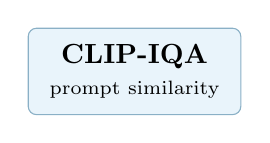
\begin{tikzpicture}\node[callout, minimum width=2.7cm, minimum height=0.85cm] {\textbf{CLIP-IQA}\\[-0.1em]\scriptsize prompt similarity};\end{tikzpicture}
  \end{column}
\end{columns}
\vfill
\flowfour{natural statistics}{distance model}{human ratings}{vision-language prompts}
\vspace{-0.15em}
{\tiny\textcolor{IQMmuted}{Sources: four primary papers. BRISQUE/NIQE practical score interpretation cross-checked with MathWorks documentation.}}
\end{frame}

% ---------- Slide 15: dataset ----------
\begin{frame}{Test dataset: TESTIMAGES 600 $\times$ 600 samples}
\begin{columns}[T,onlytextwidth]
  \begin{column}{0.62\textwidth}
    \vspace{0.05cm}
    \centering
    \fcolorbox{IQMline}{white}{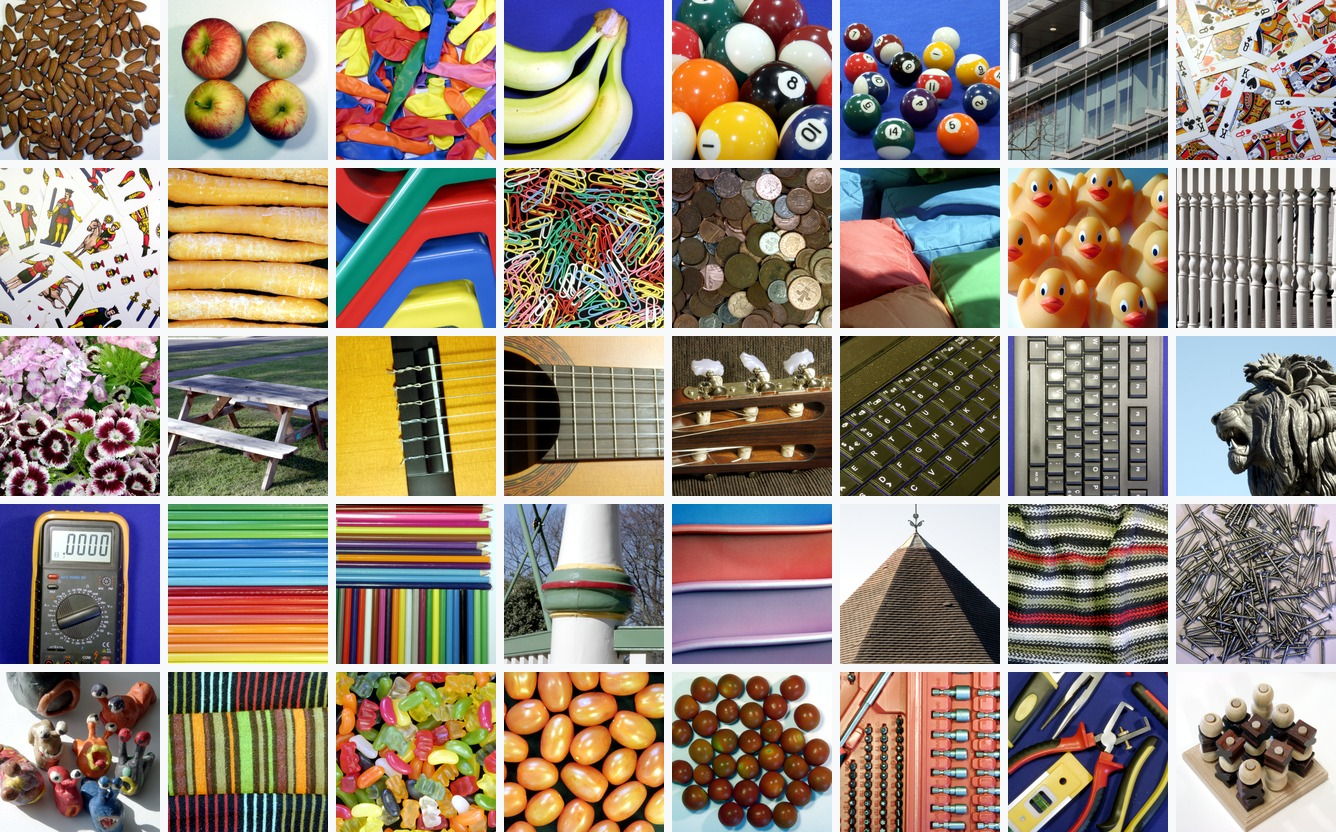
\includegraphics[width=0.96\linewidth,height=0.67\textheight,keepaspectratio]{assets/testimages_contact_sheet.jpg}}
  \end{column}
  \begin{column}{0.35\textwidth}
    \slidetag{Dataset role}
    \begin{itemize}\setlength\itemsep{0.48em}
      \item Natural scenes with varied textures, edges and colors.
      \item Used subset: \textbf{600 $\times$ 600 RGB} samples.
      \item Same images are available at multiple resolutions.
      \item Enables the same compression/IQM experiment at larger file sizes.
    \end{itemize}
    \vfill
    {\tiny\color{IQMmuted}\RaggedRight Source: testimages.org. Citation: Asuni, N., \& Giachetti, A. (2015). \emph{TESTIMAGES: A Large Data Archive for Display and Algorithm Testing}. Journal of Graphics Tools, 17(4), 113--125. DOI: 10.1080/2165347X.2015.1024298.}
  \end{column}
\end{columns}
\end{frame}

% ---------- Slide 16: src ----------
\begin{frame}{What the \texttt{src/} folder contains}
\begin{columns}[T,onlytextwidth]
\begin{column}{0.47\textwidth}
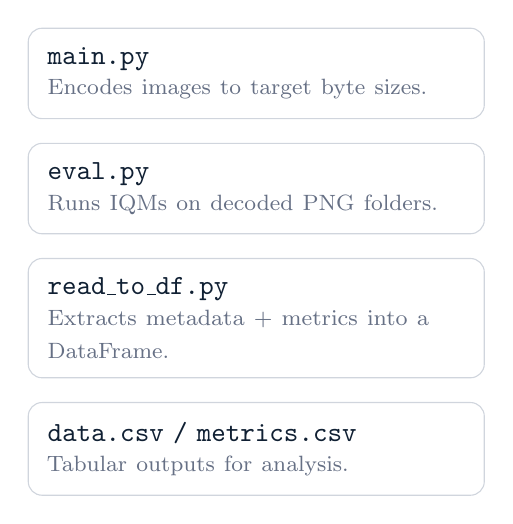
\begin{tikzpicture}[node distance=0.30cm]
\node[card, text width=5.30cm] (a) {\textbf{\texttt{main.py}}\\[-1pt]\smallmuted{Encodes images to target byte sizes.}};
\node[card, text width=5.30cm, below=of a] (b) {\textbf{\texttt{eval.py}}\\[-1pt]\smallmuted{Runs IQMs on decoded PNG folders.}};
\node[card, text width=5.30cm, below=of b] (c) {\textbf{\texttt{read\_to\_df.py}}\\[-1pt]\smallmuted{Extracts metadata + metrics into a DataFrame.}};
\node[card, text width=5.30cm, below=of c] (d) {\textbf{\texttt{data.csv / metrics.csv}}\\[-1pt]\smallmuted{Tabular outputs for analysis.}};
\end{tikzpicture}
\end{column}
\begin{column}{0.50\textwidth}
\begin{center}
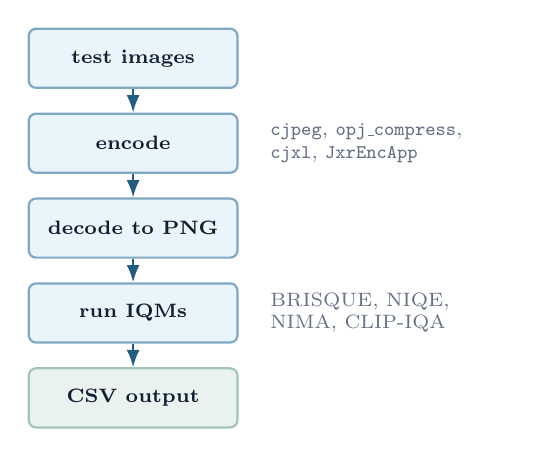
\begin{tikzpicture}[node distance=0.30cm]
\node[flowbox, minimum width=2.65cm, minimum height=0.75cm, fill=IQMaccent] (in) {test images};
\node[flowbox, minimum width=2.65cm, minimum height=0.75cm, below=of in] (enc) {encode};
\node[flowbox, minimum width=2.65cm, minimum height=0.75cm, below=of enc] (dec) {decode to PNG};
\node[flowbox, minimum width=2.65cm, minimum height=0.75cm, below=of dec] (iqm) {run IQMs};
\node[flowbox, minimum width=2.65cm, minimum height=0.75cm, below=of iqm, fill=IQMgreen!10, draw=IQMgreen!45] (csv) {CSV output};
\draw[flowarr] (in) -- (enc);
\draw[flowarr] (enc) -- (dec);
\draw[flowarr] (dec) -- (iqm);
\draw[flowarr] (iqm) -- (csv);
\node[anchor=west, text width=3.0cm, font=\scriptsize, color=IQMmuted] at ($(enc.east)+(0.28,0)$) {\texttt{cjpeg}, \texttt{opj\_compress}, \texttt{cjxl}, \texttt{JxrEncApp}};
\node[anchor=west, text width=3.0cm, font=\scriptsize, color=IQMmuted] at ($(iqm.east)+(0.28,0)$) {BRISQUE, NIQE, NIMA, CLIP-IQA};
\end{tikzpicture}
\end{center}
\end{column}
\end{columns}
\end{frame}

% ---------- Slide 17: libraries ----------
\begin{frame}{Libraries and external tools}
\begin{columns}[T,onlytextwidth]
\begin{column}{0.48\textwidth}
\slidetag{Python packages}
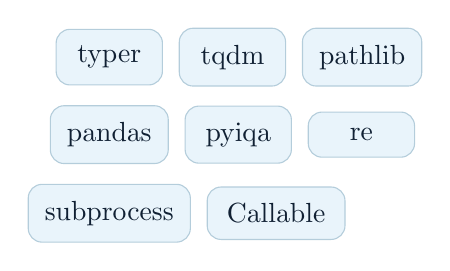
\begin{tikzpicture}[node distance=0.20cm]
\node[softcard, minimum width=1.35cm] (a) {typer};
\node[softcard, minimum width=1.35cm, right=0.20cm of a] (b) {tqdm};
\node[softcard, minimum width=1.35cm, right=0.20cm of b] (c) {pathlib};
\node[softcard, minimum width=1.35cm, below=0.25cm of a] (d) {pandas};
\node[softcard, minimum width=1.35cm, right=0.20cm of d] (e) {pyiqa};
\node[softcard, minimum width=1.35cm, right=0.20cm of e] (f) {re};
\node[softcard, minimum width=1.95cm, below=0.25cm of d] (g) {subprocess};
\node[softcard, minimum width=1.75cm, right=0.20cm of g] (h) {Callable};
\end{tikzpicture}
\vspace{0.45cm}
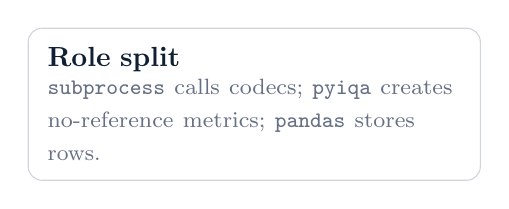
\begin{tikzpicture}
\node[card, text width=5.25cm] {\textbf{Role split}\\[-2pt]
\smallmuted{\texttt{subprocess} calls codecs; \texttt{pyiqa} creates no-reference metrics; \texttt{pandas} stores rows.}};
\end{tikzpicture}
\end{column}
\begin{column}{0.48\textwidth}
\slidetag{Codec tools / parameter modes}
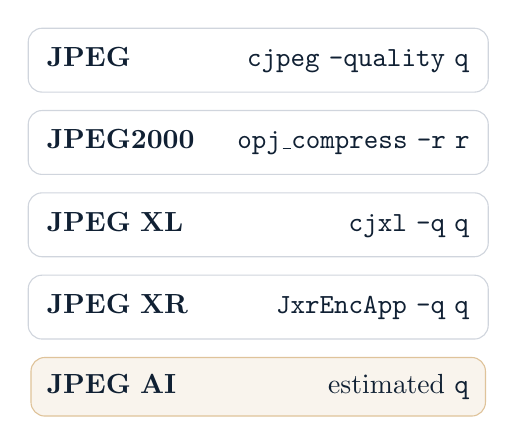
\begin{tikzpicture}[node distance=0.22cm]
\node[card, text width=5.35cm] (j) {\textbf{JPEG}\hfill \texttt{cjpeg -quality q}};
\node[card, text width=5.35cm, below=of j] (k) {\textbf{JPEG2000}\hfill \texttt{opj\_compress -r r}};
\node[card, text width=5.35cm, below=of k] (l) {\textbf{JPEG XL}\hfill \texttt{cjxl -q q}};
\node[card, text width=5.35cm, below=of l] (m) {\textbf{JPEG XR}\hfill \texttt{JxrEncApp -q q}};
\node[ambercard, text width=5.35cm, below=of m, align=left] (ai) {\textbf{JPEG AI}\hfill estimated \texttt{q}};
\end{tikzpicture}
\end{column}
\end{columns}
\end{frame}

% ---------- Slide 18: target sizes ----------
\begin{frame}[fragile]{How target sizes are defined}
\begin{columns}[T,onlytextwidth]
\begin{column}{0.50\textwidth}
\begin{lstlisting}[style=py]
FORMATS = ['jpeg', 'j2k', 'jxl', 'jxr']
SIZES = [25000, 50000, 75000,
         100000, 125000, 150000, 175000]
\end{lstlisting}
\vspace{0.25cm}
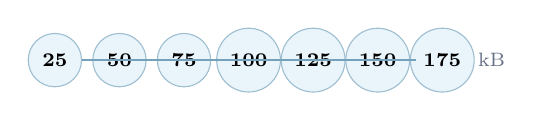
\begin{tikzpicture}
\foreach \x/\lab in {0/25,1/50,2/75,3/100,4/125,5/150,6/175}{
  \node[circle, fill=IQMaccent, draw=IQMblue!45, minimum size=0.66cm, font=\scriptsize\bfseries] at (\x*0.82,0) {\lab};
}
\draw[IQMblue!65, thick] (0.34,0) -- (4.58,0);
\node[anchor=west, font=\scriptsize, color=IQMmuted] at (5.25,0) {kB};
\end{tikzpicture}
\end{column}
\begin{column}{0.46\textwidth}
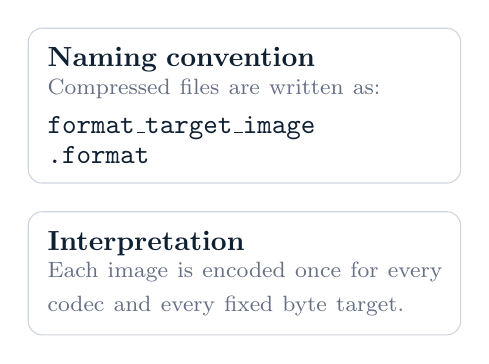
\begin{tikzpicture}[node distance=0.35cm]
\node[card, text width=5.0cm] (n) {\textbf{Naming convention}\\[-2pt]
\smallmuted{Compressed files are written as:}\\[2pt]
\texttt{format\_target\_image}\\[-1pt]\texttt{.format}};
\node[card, text width=5.0cm, below=of n] (i) {\textbf{Interpretation}\\[-2pt]
\smallmuted{Each image is encoded once for every codec and every fixed byte target.}};
\end{tikzpicture}
\end{column}
\end{columns}
\end{frame}

% ---------- Slide 19: acquired ----------
\begin{frame}[fragile]{How target sizes are acquired}
\begin{columns}[T,onlytextwidth]
\begin{column}{0.48\textwidth}

\begin{tikzpicture}
\node[softcard, text width=5.25cm, align=left] {\textbf{A) Iterative quality search}\\[-2pt]
\smallmuted{Encode, measure bytes, then narrow the quality interval.}};
\end{tikzpicture}
\vspace{0.07cm}
\begin{lstlisting}[style=py]
lo, hi = min_q, max_q
while lo + 1 < hi:
    q = (lo + hi) // 2
    bytes = encode(q)
    update_bounds(bytes, target)

encode(best_q)
\end{lstlisting}
\end{column}
\begin{column}{0.48\textwidth}
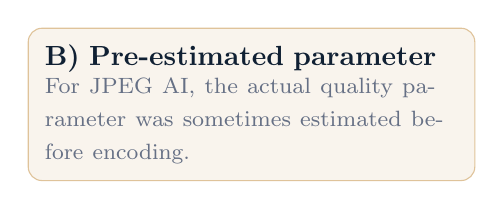
\begin{tikzpicture}
\node[ambercard, text width=5.25cm, align=left] {\textbf{B) Pre-estimated parameter}\\[-2pt]
\smallmuted{For JPEG AI, the actual quality parameter was sometimes estimated before encoding.}};
\end{tikzpicture}
\vspace{0.07cm}
\begin{lstlisting}[style=py]
q = estimate_quality(image, target)
bytes = encode_jpeg_ai(q)

if not close(bytes, target):
    refine q or rerun encode
\end{lstlisting}
\end{column}
\end{columns}
\vspace{0.20cm}

\begin{tikzpicture}
\node[card, text width=0.92\linewidth] {\textbf{Shared goal:} select a codec-specific parameter so the encoded image lands near the fixed byte target.};
\end{tikzpicture}
\end{frame}

% ---------- Slide 20: IQMS in code ----------
\begin{frame}[fragile]{No-reference IQMs in the code}
\begin{columns}[T,onlytextwidth]
\begin{column}{0.52\textwidth}
\begin{lstlisting}[style=py]
IQMS = {
  'brisque': pyiqa.create_metric('brisque'),
  'niqe':    pyiqa.create_metric('niqe'),
  'nima':    pyiqa.create_metric('nima'),
  'clip':    pyiqa.create_metric('clipiqa')
}

score = metric(str(img_path)).item()
\end{lstlisting}
\end{column}
\begin{column}{0.44\textwidth}
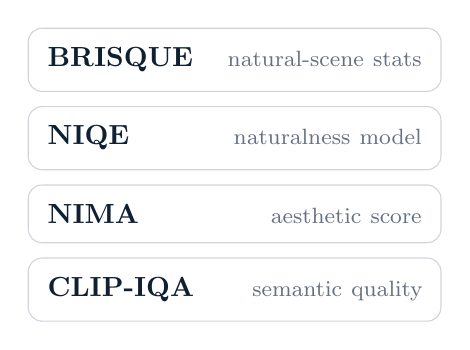
\begin{tikzpicture}[node distance=0.18cm]
\node[card, text width=4.75cm] (bq) {\textbf{BRISQUE}\hfill \smallmuted{natural-scene stats}};
\node[card, text width=4.75cm, below=of bq] (nq) {\textbf{NIQE}\hfill \smallmuted{naturalness model}};
\node[card, text width=4.75cm, below=of nq] (nm) {\textbf{NIMA}\hfill \smallmuted{aesthetic score}};
\node[card, text width=4.75cm, below=of nm] (ci) {\textbf{CLIP-IQA}\hfill \smallmuted{semantic quality}};
\end{tikzpicture}
\vspace{0.18cm}
\smallmuted{Applied to decoded PNG images - no reference image required.}
\end{column}
\end{columns}
\end{frame}

% ---------- Slide 21: evaluation rows ----------
\begin{frame}[fragile]{Evaluation loop and CSV rows}
\begin{columns}[T,onlytextwidth]
\begin{column}{0.53\textwidth}
\begin{lstlisting}[style=py]
for fmt in FORMATS:
  for size in SIZES:
    for img in decoded_folder.glob('*.png'):
      row = {
        'image_id': img.stem,
        'format': fmt,
        'target_size': size
      }
      for name, metric in IQMS.items():
        row[name] = metric(str(img)).item()
      data_rows.append(row)
\end{lstlisting}
\end{column}
\begin{column}{0.43\textwidth}
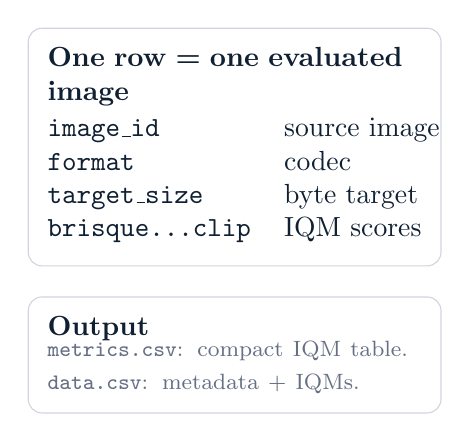
\begin{tikzpicture}[node distance=0.38cm]
\node[card, text width=4.75cm] (row) {\textbf{One row = one evaluated image}\\[2pt]
\begin{tabular}{@{}ll@{}}
\texttt{image\_id} & source image \\
\texttt{format} & codec \\
\texttt{target\_size} & byte target \\
\texttt{brisque...clip} & IQM scores
\end{tabular}};
\node[card, text width=4.75cm, below=of row] (out) {\textbf{Output}\\[-2pt]\smallmuted{\texttt{metrics.csv}: compact IQM table.\\\texttt{data.csv}: metadata + IQMs.}};
\end{tikzpicture}
\end{column}
\end{columns}
\end{frame}

% ---------- Slide 22: results placeholder ----------
\begin{frame}{Results: codec comparison}
\begin{center}
\vspace{0.6cm}

\begin{tikzpicture}[node distance=0.42cm]
  \node[softcard, text width=3.35cm, minimum height=1.05cm] (a) {\textbf{Rows}\\[-0.1em]\scriptsize image $\times$ codec $\times$ size};
  \node[softcard, text width=3.35cm, minimum height=1.05cm, right=of a] (b) {\textbf{Aggregation}\\[-0.1em]\scriptsize mean / spread per codec};
  \node[greencard, text width=3.35cm, minimum height=1.05cm, right=of b] (c) {\textbf{Result view}\\[-0.1em]\scriptsize best codec per target size};
  \draw[flowarr] (a) -- (b); \draw[flowarr] (b) -- (c);
\end{tikzpicture}
\vspace{0.8cm}

\begin{tikzpicture}
  \node[card, text width=0.78\linewidth, align=center, minimum height=1.2cm] {\Large\textcolor{IQMmuted}{Placeholder for result plots}};
\end{tikzpicture}
\end{center}
\end{frame}

% ---------- Slide 23: results placeholder ----------
\begin{frame}{Results: IQM behavior}
\begin{columns}[T,onlytextwidth]
\begin{column}{0.50\textwidth}

\begin{tikzpicture}
\node[card, text width=5.45cm, minimum height=4.5cm, align=center] {\Large\textcolor{IQMmuted}{Placeholder}\\[0.4em]\smallmuted{BRISQUE / NIQE trends}};
\end{tikzpicture}
\end{column}
\begin{column}{0.46\textwidth}

\begin{tikzpicture}
\node[card, text width=5.05cm, minimum height=4.5cm, align=center] {\Large\textcolor{IQMmuted}{Placeholder}\\[0.4em]\smallmuted{NIMA / CLIP-IQA trends}};
\end{tikzpicture}
\end{column}
\end{columns}
\end{frame}

% ---------- Slide 24: results placeholder ----------
\begin{frame}{Results: takeaway placeholder}
\begin{center}
\vspace{0.55cm}

\begin{tikzpicture}[node distance=0.55cm]
\node[softcard, text width=3.3cm, minimum height=1.15cm] (a) {\textbf{Controlled}\\[-0.1em]\scriptsize fixed target sizes};
\node[softcard, text width=3.3cm, minimum height=1.15cm, right=of a] (b) {\textbf{Compared}\\[-0.1em]\scriptsize compression standards};
\node[greencard, text width=3.3cm, minimum height=1.15cm, right=of b] (c) {\textbf{Measured}\\[-0.1em]\scriptsize no-reference scores};
\draw[flowarr] (a) -- (b); \draw[flowarr] (b) -- (c);
\end{tikzpicture}
\vspace{0.75cm}

\begin{tikzpicture}
\node[card, text width=0.80\linewidth, align=center, minimum height=1.45cm] {\Large\textcolor{IQMmuted}{Final findings will be inserted here}};
\end{tikzpicture}
\end{center}
\end{frame}

\end{document}
